\documentclass[tikz,border=12pt]{standalone}
\usepackage[utf8]{inputenc}
\usepackage[T1]{fontenc}
\usepackage{helvet}
\renewcommand{\familydefault}{\sfdefault}
\usetikzlibrary{arrows.meta,calc}

\tikzset{
	src/.style={draw=black, rounded corners=4pt, fill=gray!65, text=white,
		minimum width=2.1cm, minimum height=0.62cm, line width=0.6pt},
	tgt/.style={draw=black, rounded corners=4pt, fill=gray!15, text=black,
		minimum width=2.1cm, minimum height=0.62cm, line width=0.6pt},
	note/.style={font=\bfseries\small, align=center},
	arr/.style={-{Stealth[length=2.6mm]}, line width=0.8pt},
}

\newcommand{\dx}{2.4}

\begin{document}
	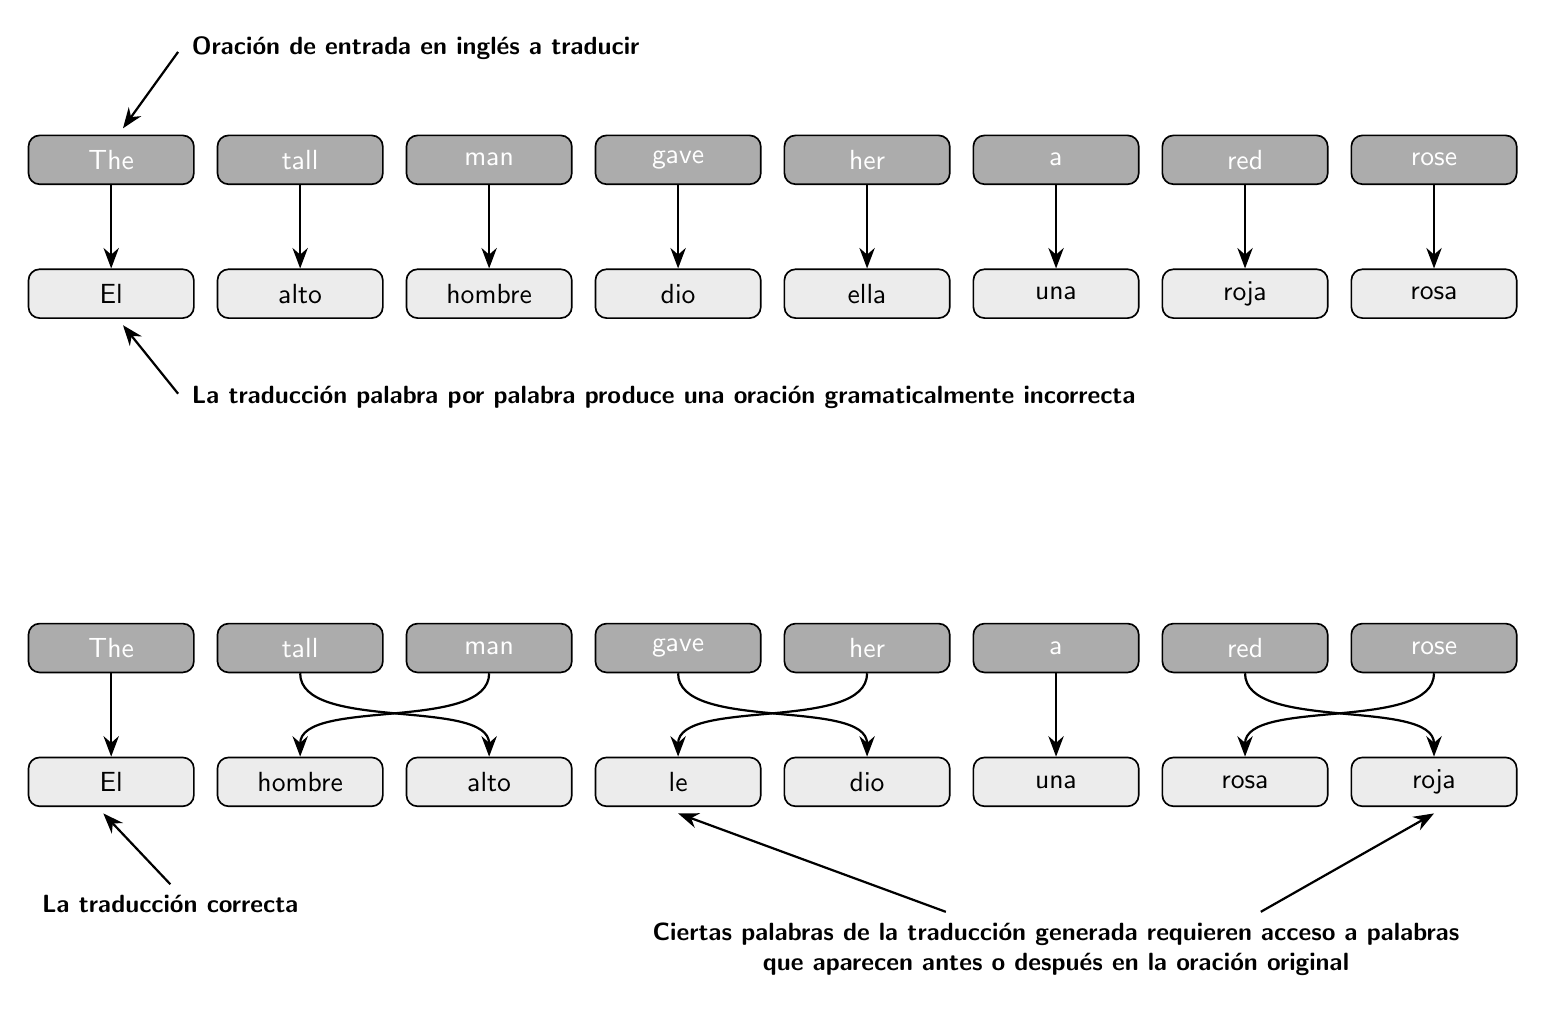
\begin{tikzpicture}
		
		%% ===================== Panel superior: palabra por palabra =====================
		\foreach \w [count=\i] in {The,tall,man,gave,her,a,red,rose}
		\node[src] (a\i) at (\i*\dx,0) {\w};
		\foreach \w [count=\i] in {El,alto,hombre,dio,ella,una,roja,rosa}
		\node[tgt] (b\i) at (\i*\dx,-1.7) {\w};
		\foreach \i in {1,...,8}
		\draw[arr] (a\i.south) -- (b\i.north);
		
		\node[note, anchor=west] (n1) at ($(a1.north)+(0.9,1.1)$)
		{Oración de entrada en inglés a traducir};
		\draw[arr] ($(n1.west)+(-0.05,-0.05)$) -- ($(a1.north)+(0.15,0.08)$);
		
		\node[note, anchor=west] (n2) at ($(b1.south)+(0.9,-1.0)$)
		{La traducción palabra por palabra produce una oración gramaticalmente incorrecta};
		\draw[arr] ($(n2.west)+(-0.05,0.05)$) -- ($(b1.south)+(0.15,-0.08)$);
		
		%% ===================== Panel inferior: traducción correcta =====================
		\def\yo{-6.2}
		\foreach \w [count=\i] in {The,tall,man,gave,her,a,red,rose}
		\node[src] (c\i) at (\i*\dx,\yo) {\w};
		\foreach \w [count=\i] in {El,hombre,alto,le,dio,una,rosa,roja}
		\node[tgt] (d\i) at (\i*\dx,\yo-1.7) {\w};
		
		% Alineación: The->El, tall->alto, man->hombre, gave->dio,
		%             her->le, a->una, red->roja, rose->rosa
		\draw[arr] (c1.south) -- (d1.north);
		\draw[arr] (c6.south) -- (d6.north);
		\foreach \s/\t in {2/3, 3/2, 4/5, 5/4, 7/8, 8/7}
		\draw[arr] (c\s.south) .. controls +(0,-0.75) and +(0,0.75) .. (d\t.north);
		
		\node[note, anchor=north west] (n3) at ($(d1.south)+(-1.0,-1.0)$)
		{La traducción correcta};
		\draw[arr] ($(n3.north)+(0,0.02)$) -- ($(d1.south)+(-0.1,-0.08)$);
		
		\node[note, anchor=north] (n4) at ($(d6.south)+(0,-1.35)$)
		{Ciertas palabras de la traducción generada requieren acceso a palabras\\
			que aparecen antes o después en la oración original};
		\draw[arr] ($(n4.north)+(-1.4,0.02)$) -- ($(d4.south)+(0,-0.08)$);
		\draw[arr] ($(n4.north)+(2.6,0.02)$)  -- ($(d8.south)+(0,-0.08)$);
		
	\end{tikzpicture}
\end{document}